\section{Design}
This section covers both game design and software architecture design, as well as the
design of the individual software modules.

\subsection{Game Design}
The game is an arkanoid clone and as such it is very simple and follows the general arkanoid formula of destroying
bricks using a ball that bounces around the screen. The ball will reflect itself off of a brick, wall
in the top of the playing space as well as two walls bordering the sides of the playing space.
There is nothing stopping at the bottom of the playing space, except the player controlled striker.
It is the players objective to control the striker such that the ball is reflected off of it and
hits all the bricks. Thereby destroying the bricks. \\

In this version of arkanoid, which we will henceforth refer to as Smashing Bricks, the player
upon starting a game is presented with a splash screen, followed by the first level. The levels
themselves contain a brick layout that can be changed as well as a monochrome background image.
Upon completion of the level, the full-color background image is revealed and the player can
move on to the next level. Once the player reaches the end of the game, the players score
will be presented and the option to restart the game will be available. \\

The score is incremented by a set amount every time a brick is hit or destroyed. If the player
misses the ball, another amount is subtracted from the score. If the players score goes below
0, the game is over and the player will have the option to restart the game. \\

The balls reflection from the striker is not actually a reflection, instead the direction
of the ball is changed according to where it hit the striker. As with all games, these
mechanics are based on their feeling and this to us felt like the most natural way to play.
Similarly the speed of the ball and striker are also based on feel. \\

Background music will play and sound effects are triggered every time the ball is reflected
from a brick, a wall or the striker. \\

The game only has a single difficulty, hard, this is due to the fact that we deemed slow and/or
easy arkanoid games to get boring too quickly. The game is therefore deliberately designed to 
force the player to quickly be able to estimate where the ball will reach the bottom again, as 
soon as it leaves the striker.

\subsection{Software Architecture Design}
Considerable time and effort went into insuring that the software itself would be modular and easily extensible.
As mandated, the software contains three layers. A hardware layer that is concerned only with
direct hardware manipulations, an API layer that is concerned with presenting general functionality to
the final application layer. The layers can be changed individually as long as they present the
same functionality to the layer directly above. \\

In our design, the hardware layer is relatively small as it only needs to deal with the following:

\begin{itemize}
	\item Handle ADC input for the joystick.
	\item Set up timers.
	\item Send data over SPI.
\end{itemize}

It is not necessary to write software that controls the UART as API functions covering  this
 is already provided by the default eZ8 libraries included in ZDS. \\

The API functions needed for general game applications are then the following.

\begin{itemize}
	\item Graphics.
	\item Sound.
	\item Math. (Sine, Cosine, fix point etc.)
	\item Input handling.
\end{itemize}

The API layer presents a general framework that can be used for any game application. If extra
functionality is needed it is also easily extensible. \\

To make the game application itself as modular and extensible as possible, we have utilized a
style of C programming that approaches object oriented programming as this is especially well
suited for games. To understand why, we must look at the general game application control flow. \\

Modern games run either with a fixed or a free running framerate, we will only discuss the fixed
framerate type as this is easier to work with for this application. Within every frame period, the
game situation is updated. This means getting input from the user and  updating the position of every object
, checking collisions and reacting accordingly etc. When this is done, the new situation is presented to the
 user by updating the graphics medium, in this case a terminal. The cycle then repeats until the game
ends. This can be split into 3 distinct operations that need to be performed within the main game loop:
Get input, update, render. \\

The advantage of object oriented programming is that all game entities can then contain their own
update and render functions, eliminating the need to change exisiting code when a new game entity is added.
This also helps to avoid spaghetti code and deep nesting problems. While we are aware that object oriented
programming usually comes with significant performance overhead and as such is not suitable for a microprocessor,
we deem this to not be a problem as we do not use truly object oriented style, only an approximate one, where every
entity is represented as a struct with function pointers to its inner "methods" and primitives for fields.
Only a small amount of glue code is needed to control the transition between levels and manage the game state. \\

Communication between modules follows the mantra that less is good. As such, the amount of information and functions
present to each other is kept at a minimum. This is done to keep the number of entry points to a module as small
as possible, thus making it possible to change the inner workings of a module without breaking external dependencies.
As functions and variables in C are confined to their own scope, the file in which they are declared, and this
scope can only be extended by including them in a header file, our header files are kept as simple as possible. \\

A block diagram of the modules and their communication paths can be seen in figure \ref{architecture_block}

\begin{figure}
	\center
	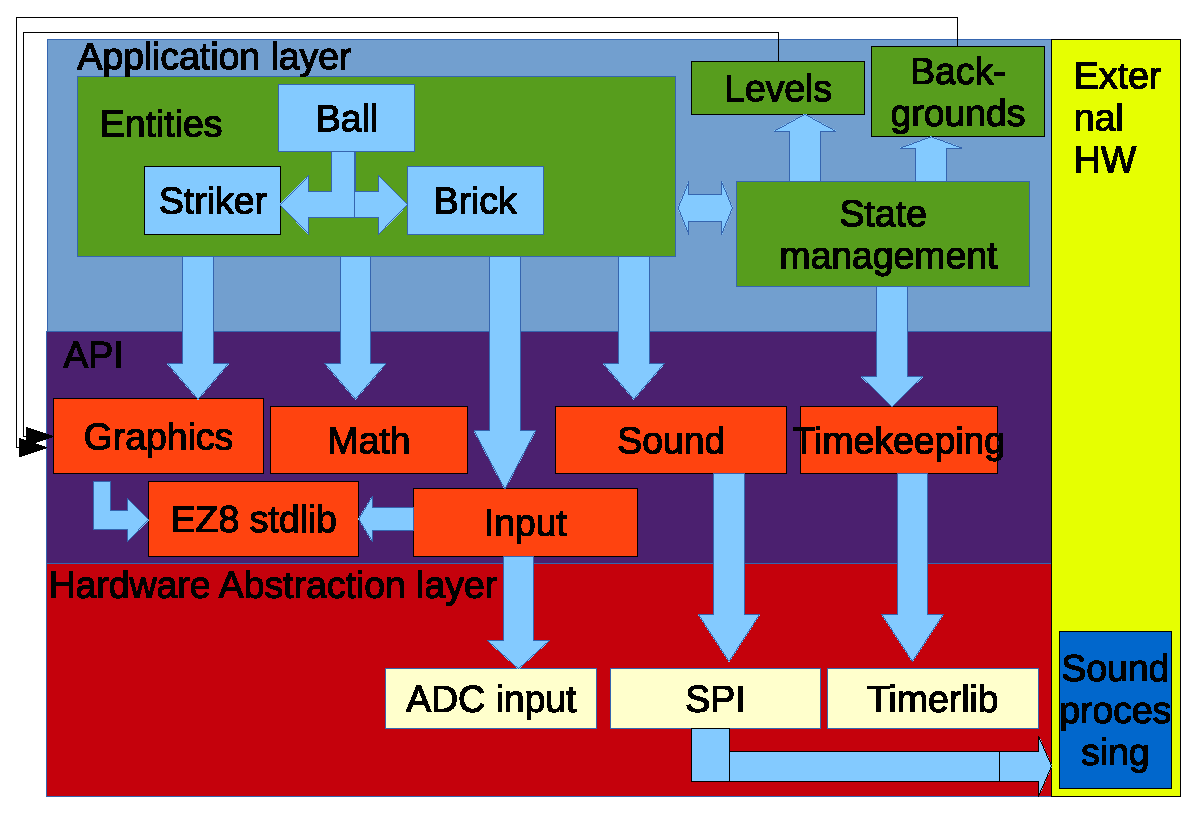
\includegraphics[scale=0.7]{pictures/architecture_block.eps}
	\caption{Block diagram of the software modules and their communication}
	\label{architecture_block}
\end{figure}
